
\documentclass[12pt]{article} % Use A4 paper with a 12pt font size - different paper sizes will require manual recalculation of page margins and border positions

% Generated with LaTeXDraw 2.0.8
% Mon Jun 17 19:00:40 EDT 2013
\usepackage[usenames,dvipsnames]{pstricks}
\usepackage{epsfig}

\usepackage{pst-grad} % For gradients
\usepackage{pst-plot} % For axes
\usepackage[left=1.3cm,right=4.6cm,top=1.8cm,bottom=4.0cm,marginparwidth=3.4cm]{geometry} % Adjust page margins
\usepackage{amsmath} % Required for equation customization
\usepackage{amssymb} % Required to include mathematical symbols
\usepackage{xcolor} % Required to specify colors by name
\usepackage{amsthm}
\usepackage{float}
\usepackage{tikz}
\usepackage{pgfplots}
\usetikzlibrary{shapes,backgrounds,trees}
\usepackage{wasysym}
\usepackage{scrextend}
\makeatletter
\newcommand{\infi}{\int_{-\infty}^\infty}
\newcommand{\mytag}[2]{%
  \text{#1}%
  \@bsphack
  \protected@write\@auxout{}%
         {\string\newlabel{#2}{{#1}{\thepage}}}%
  \@esphack
}
\makeatother

\setlength{\parindent}{0cm} % Remove paragraph indentation
\newcommand{\tab}{\hspace*{2em}} % Defines a new command for some horizontal space
%\newcommand{\choose}[2]{\left(\begin{matrix}
%{#1}\\{#2}
%\end{matrix}\right)}
\date{}
\title{Introduction to Probability Theory - Lecture 22}
%----------------------------------------------------------------------------------------
\newcommand{\pdf}[2]{\left\{\begin{matrix}
{#1} & {#2}\\\\\\0&\textrm{otherwise}
\end{matrix}\right.}
\newtheorem{defn}{Definition}
\newtheorem{example}{Example}
\newtheorem{prop}{Proposition}
\newtheorem{exer}{Exercises}
\newtheorem{thm}{Therorem}

\begin{document}
\maketitle

\section{Transformations}
We have already seen that if $g(x)$ is a function and $X$ is a random varible, then $Y= g(X)$ is also a random variable. Our goal now is to find the corresponding distribution of the transformed random variable. As usual, we begin with the discrete case.

\subsection{Transformations of Discrete Random Variables}
Let $X$ be a random variable, $g(x)$ a function and let $Y=g(X)$. Then:
$$P(Y=y) = P(g(X) = y) = \sum_{x:g(x)=y} P(X=x)$$
where the sum is over each value of $x$ that is mapped to $y$ under $g(x)$. What does this mean?
\paragraph{Aside on Functions and Inverses}
Many students learn about inverse functions in calculus - but often what they seem to take away from it has to do with the mechanics of computing the inverse rather than what the inverse actually \emph{is}. "That thing where you solve for $x$ and then change $x$ to $y$" is a common recollection. But the inverse itself is the function you find. We'll need a few preliminary definitions and then we'll formally define the inverse.\\

First, it is important to fully understand what a \emph{function} is: A function
$$f:\mathbb{R}\rightarrow\mathbb{R}$$
takes a real number ($\mathbb{R}$ stands for 'the real numbers') and returns a real number. The input is often denoted $x$, and $f(x)$ is the resulting number. When we graph a function on axes labeled $x$ and $y$, we usually write: $y=f(x)$. In the plot, each value of $x$ is assigned to a value $f(x)$ that is plotted on the $y$ axis. For example:


\begin{tikzpicture}
  \begin{axis}[ 
    xlabel=$x$,
    ylabel={$y = f(x) = x^2$}
  ] 
    \addplot[samples=700,thick] {x^2}; 
  \end{axis}
\end{tikzpicture} 

The function in the above figure does not assign \emph{unique} $y$ values to each $x$. In fact, other than at the point $x=0$, each value of $y$ corresponds to \emph{two} input values $x$. \\\\
Now, suppose I give you a value $y$ and ask what value $x$ do I need to give to $f$ to obtain $y$? This would be a problem for any $y\neq 0$, because each $y$ is assigned to two different values of $x$.\\\\
Now, consider another function:

\begin{tikzpicture}
  \begin{axis}[ 
    xlabel=$x$,
    ylabel={$y = f(x) = x^3$}
  ] 
    \addplot[samples=700,thick] {x^3}; 
  \end{axis}
\end{tikzpicture} 

This function is different. Each $y$ value originates from a unique $x$ value. If I say, $y=-8$, what value of $x$ gives $f(x) = -8$, you can tell me: $x=-2$. This function is said to be \emph{one-to-one}. It is also \emph{invertible}! When a function is invertible, we can play the game 'find-the-x-that-y-came-from'. Let's formalize some of this:\\\\

\begin{defn}

A function $f$ is one-to-one $\iff$ 
$$f(x_1)=f(x_2) \Rightarrow x_1=x_2$$
In other words, each $x$ in the domain is mapped to a unique $y$ in the range.

\end{defn}

Note that a one-to-one function must either be strictly increasing $x_1<x_2 \iff f(x_1)<f(x_2)$ or strictly decreasing ($x_1<x_2\iff f(x_1)>f(x_2)$. 

\begin{defn}
Let $f:\mathbb{R}\rightarrow\mathbb{R}$ and suppose there exists $f^{-1}(x)$ such that 
$$f^{-1}(f(x)) = x$$.
Then $f^{-1}$ is called the \emph{inverse} of $f$ and $f$ is said to be \emph{invertible}.
\end{defn}

You have already met functions who are inverses of one another. For example, $log(x)$ and $e^x$, or $x^3$ and $x^{\frac13}$. Note that inverse is a symmetric property. In other words, if $g$ is the inverse of $f$, then $f$ is the inverse of $g$. Also, if $f$ is strictly increasing/decreasing then it's inverse is strictly increasing/decreasing. We will use this fact explicitly when we are defining CDFs of random variables that are transformed via an invertible function.

Now, just a final note: although a function may very well return the same value of $y$ for many different inputs $x$, a function \emph{must} map each input $x$ to only one value. 

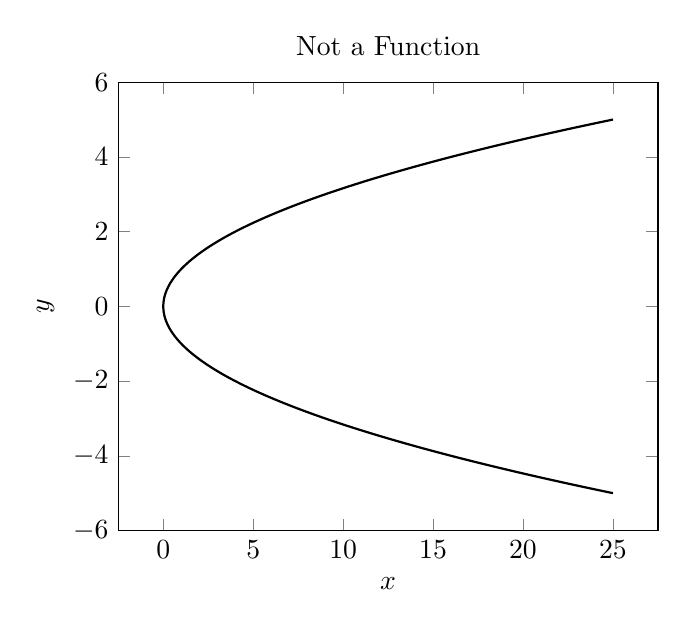
\begin{tikzpicture}
  \begin{axis}[ 
   title=Not a Function,
    xlabel=$x$,
    ylabel={$y$}
  ] 
    \addplot[samples=700,thick] ({x^2},{x}); 
  \end{axis}
\end{tikzpicture} 

\paragraph{Finished Aside}

Returning to our transformed random variable, $Y=g(X)$,
$$P(Y=y) = P(g(X) = y) = \sum_{x:g(x)=y} P(X=x)$$
means to obtain the probability that $Y$ takes a value $y$, we must sum the probability that $X$ takes the value $x$ for each $x$ that results in $g(x) = y$. For example, if $g(x) = x^2$, then 
$$P(Y=4) = P(X=2) + P(X=-2)$$
In the case of an invertible function $g(x)$, we can compute:
$$P(Y=y) = P(g^{-1}(Y)=g^{-1}(y)) = P(X = x)$$
(where $x=g^{-1}(y)$).

\subsection{Transformations of Continuous Random Variables}
In the discrete case, finding the pmf of a transformed variable is very straightforward. If the function is invertible, we just apply the inverse of the function to the pmf, and we are done. If the function is not invertible, we just sum $P(X=x)$ over all the values of $x$ for which $g(x) = y$. In the continuous case, we have a slight complication: probability is determined by integrating the pdf over an interval - so transforming the random variable leads to a change of variable of integration.\\\\
\paragraph{Change of Variables}
\begin{thm}
Let $X$ be a continuous random variable with pdf $f(x)$. Let $Y=g(X)$, where $g$ is differentiable and 1-1 (in other words, invertible). Then the pdf of $Y$ is
$$f_Y(y)= f_X(x)\left|\frac{dx}{dy}\right|$$
where $x=g^{-1}(y)$ and the support of $f_Y(y)$ is given by $\left\{g(x): x\in \mathrm{supp}(X)\right\}$
\end{thm} 
\begin{proof}
If $g$ is 1-1, it is either increasing or decreasing. Suppose $f$ is increasing. The CDF
$$F_Y(y) = P(Y\leq y) = P(g(X)\leq y) = P(g^{-1}(g(X))\leq g^{-1}(y)) = F_X(g^{-1}(y)$$
Now, differentiate to get the pdf:
$$\frac{d}{dy} F_Y(y) = \frac{d}{dy} \left[F_X(g^{-1}(y)\right] = \left.\frac{dF_x}{dy}\right\rvert_{g^{-1}(y)} \frac{d}{dy} g^{-1}(y) = f_x(x) \frac{dx}{dy}$$
Now, because we assumed $g$ to be increasing, $g^{-1}$ is increasing, and $\frac{dg^{-1}}{dy}$ is positive, so:
$$\frac{d}{dy} F_Y(y)f_X(x)\left|\frac{dx}{dy}\right|$$
If $g$ is decreasing, the same argument yields 
$$f_Y(y) = -f_X(x)\frac{dx}{dy}$$
and $\frac{dx}{dy}$ is negative, so we obtain:
$$f_Y(y) = f_X(x)\left|\frac{dx}{dy}\right|$$
\end{proof}
All we have really done is proved the change of variables formula for an integral! Let's do an example:
\begin{example}
Let $X$ be a continuous random variable with pdf:
$$f_X(x) = \pdf{\frac{2}{x^3}}{1<x<\infty}$$
What is the pdf of $Y=e^X$?\\\\
Recall that $\log$ is the inverse of the exponential, so:
$$y=e^x\iff x=\log(y)$$
and we compute:
$$\frac{dx}{dy} = \frac1x$$
so that:
$$f_Y(y) = f_X(x)\left|\frac{dx}{dy}\right| = f_X(\log(y))\frac1y = \frac1y\frac2{\left(\log(y)\right)^3} = \frac2{y\left(\log(y)\right)^3}$$
and because $y=e^x$ and $0<x<\infty$, the support of $f_Y(y)$ is $e<y<\infty$.
\end{example}
\paragraph{CDF Method}
Now, what if the transformation is not invertible? When this is the case, we can sometimes use 'the CDF technique'. Let $X$ be a continuous random variable and suppose $Y=u(X)$ for some function $u(x)$. Consider the CDF of $Y$:
$$F_Y(y) = P(Y\leq y) = P(u(X)\leq y)$$
Usually, we can write:
$$P(u(X)\leq y) = P(x_1 \leq X \leq x_2)$$
where $x_1$ and $x_2$ are functions of $y$. Thus,
$$F_Y(y) = \int_{x_1(y)}^{x_2(y)} f_X(x) dx$$
and then recover the pdf by differentiation:
$$f_Y(y) = \frac{d}{dy} F_Y(y)$$
Let's see an example of this:\\
\begin{example}
Let $X$ be a continuous random variable with pdf $f_X(x)$ and CDF $F_X(x)$. Define $Y=X^2$.
$$F_Y(y) = P(Y\leq y) = P(X^2\leq y) = P(-\sqrt{y} \leq X\leq \sqrt{y}$$
$$= F_X(\sqrt{y}) - F_X(-\sqrt{y})$$
Thus,
$$f_Y(y) = \frac{d}{dy} F_Y(y) = \frac{d}{dy}\left[F_X(\sqrt{y})-F_X(-\sqrt{y})\right]$$
$$= \frac1{2\sqrt{y}}F_X'(\sqrt{y}) + \frac1{2\sqrt{y}}F_X'(-\sqrt{y}) =  \frac1{2\sqrt{y}}\left(f_x(\sqrt{y})+f_X(-\sqrt{y})\right)$$
and because $Y$ = $X^2$, $y>0$.
\end{example}
\paragraph{MGF Method}
There is one more way to find the pdf (or even pmf in the case of a discrete random variable) of a transformed random variable. Recall that the moment generating function is unique, in the sense that two random variables with the same MGF have the same distribution. If we can somehow compute the MGF of a transformed random variable, and we can recognize it as the MGF of a known distribution, we know the pdf.\\\\
\begin{example}
Let $X_1,...,X_k$ be independent binomial random variables with $X_i\sim Bin(n_i,p)$. Let
$$Y=\sum_{i=1}^k X_i$$
Then
$$M_Y(t) = M_{X_1+...+M_k}(t) = M_{X_1}(t)\cdots M_{X_k}(t)$$
$$ = \left(pe^t + q\right)^{n_1}\cdots\left(pe^t+q\right)^{n_k} = \left(pe^t + q\right)^{n_1+...+n+k} $$
and this is the MGF for a random variable that has the binomial distribution with success probability $p$ and $n+1+...+n_k$ trials. So $Y\sim Bin(n_1+...+n_k,p)$.
\end{example}
Here is one more example:
\begin{example}
Let $X_i$ be iid $\sim Pois(\mu_i)$ and define $Y_i=\sum_{i=1}^k X_i$.
For each $i$,
$$M_{X_i}(t) = \exp(\mu_i(e^t-1))$$
so 
$$M_Y(t) = \exp(\mu_1(e^t-1))\cdots\exp(\mu_k(e^t-1))= \exp((\mu_1+...+\mu_k)r^t-1))$$
which is the pdf of a Poisson random variable with parameter $\mu = \mu_1+...+\mu_k$.
\end{example}
\subsection{Transformations of Continuous Multivariable Random Variables}
We have seen that in the single-variable continuous case, our change of variables formula requires the absolute value of the derivative of the inverse of the transformation function. In the multivariable case, we need to compute the matrix of first partial derivatives (called the Jacobian) of the inverse transformation.\\\\
We consider only the 2-dimensional case and note that the computations generalize easily to arbitrary dimension. Suppose $u_1$ and $u_2$ are functions of $x_1$ and $x_2$. Let 
$$y_1 = u_1(x_1,x_2) \;\;\;\textrm{ and }\;\;\; y_2 = u_2(x_1,x_2)$$
Then if we can solve for $x_1$ and $x_2$, so that:
$$x_1 = v_1(y_1,y_2)  \;\;\;\textrm{ and }\;\;\; x_2 = v_2(y_1,y_2)$$
Then the Jacobian is:
$$\left(\begin{matrix}
\frac{\partial x_1}{\partial y_1} &\frac{\partial x_1}{\partial y_2} \\
\frac{\partial x_2}{\partial y_1} &\frac{\partial x_2}{\partial y_2} 
\end{matrix}\right)$$
For our change of variables formula, we will need the absolute value of the \emph{determinant} of the Jacobian:
$$\mathcal{J} = \left|\begin{matrix}
\frac{\partial x_1}{\partial y_1} &\frac{\partial x_1}{\partial y_2} \\
\frac{\partial x_2}{\partial y_1} &\frac{\partial x_2}{\partial y_2} 
\end{matrix}\right| = \left|\frac{\partial x_1}{\partial y_1}\cdot\frac{\partial x_2}{\partial y_2} -  \frac{\partial x_2}{\partial y_1}\cdot \frac{\partial x_1}{\partial y_2}\right|$$
\begin{example}
Consider the transformation 
$$y_1 = x_1$$
$$y_2 = x_1x_2$$
so that the inverse is:
$$x_1 = y_1$$
$$x_2=\frac{y_2}{y_1}$$
We compute:
$$\mathcal{J} = \left|\begin{matrix}
\frac{\partial x_1}{\partial y_1} &\frac{\partial x_1}{\partial y_2} \\
\frac{\partial x_2}{\partial y_1} &\frac{\partial x_2}{\partial y_2} 
\end{matrix}\right| = \left|\begin{matrix}
1 & 0 \\
\frac{-y_2}{y_1^2} &\frac{1}{\partial y_1^2} 
\end{matrix}\right|$$
\end{example}
In general, the Jacobian in $n$ dimensions is an $n\times n$ matrix. We now present the change of variables formula for a joint pdf of two random variables.\\

\begin{thm}
Let $X=(X_1,X_2)$ and $Y= (Y_1,Y_2) =g(X)$ for some invertible function $g(x)$. (By invertible, we mean that we can solve for $x_1$ and $x_2$ in terms of $y_1$ and $y_2$.) Suppose
$$x_1 = h_1(y_1,y_2) \;\;\; \mathrm{ and } \;\;\; x_2=h_2(y_1,y_2)$$
Then
$$\mathcal{J} = \left|\begin{matrix}
\frac{\partial x_1}{\partial y_1} &\frac{\partial x_1}{\partial y_2} \\
\frac{\partial x_2}{\partial y_1} &\frac{\partial x_2}{\partial y_2} 
\end{matrix}\right| = \left|\frac{\partial x_1}{\partial y_1}\cdot\frac{\partial x_2}{\partial y_2} -  \frac{\partial x_2}{\partial y_1}\cdot \frac{\partial x_1}{\partial y_2}\right|$$
and (if $g$ is invertible) $\mathcal{J} \neq 0$. Then the pdf of $Y$ is given by
$$f_Y(y_1,y_2) = f_X(X_1,X_2) \mathcal{J}$$
where $f_X(x_1,x_2)$ is the pdf of $X$.
\end{thm}
\end{document}